% Options for packages loaded elsewhere
\PassOptionsToPackage{unicode}{hyperref}
\PassOptionsToPackage{hyphens}{url}
\PassOptionsToPackage{dvipsnames,svgnames,x11names}{xcolor}
%
\documentclass[
  12pt,
]{article}
\usepackage{amsmath,amssymb}
\usepackage{lmodern}
\usepackage{iftex}
\ifPDFTeX
  \usepackage[T1]{fontenc}
  \usepackage[utf8]{inputenc}
  \usepackage{textcomp} % provide euro and other symbols
\else % if luatex or xetex
  \usepackage{unicode-math}
  \defaultfontfeatures{Scale=MatchLowercase}
  \defaultfontfeatures[\rmfamily]{Ligatures=TeX,Scale=1}
\fi
% Use upquote if available, for straight quotes in verbatim environments
\IfFileExists{upquote.sty}{\usepackage{upquote}}{}
\IfFileExists{microtype.sty}{% use microtype if available
  \usepackage[]{microtype}
  \UseMicrotypeSet[protrusion]{basicmath} % disable protrusion for tt fonts
}{}
\makeatletter
\@ifundefined{KOMAClassName}{% if non-KOMA class
  \IfFileExists{parskip.sty}{%
    \usepackage{parskip}
  }{% else
    \setlength{\parindent}{0pt}
    \setlength{\parskip}{6pt plus 2pt minus 1pt}}
}{% if KOMA class
  \KOMAoptions{parskip=half}}
\makeatother
\usepackage{xcolor}
\usepackage[margin=1in]{geometry}
\usepackage{longtable,booktabs,array}
\usepackage{calc} % for calculating minipage widths
% Correct order of tables after \paragraph or \subparagraph
\usepackage{etoolbox}
\makeatletter
\patchcmd\longtable{\par}{\if@noskipsec\mbox{}\fi\par}{}{}
\makeatother
% Allow footnotes in longtable head/foot
\IfFileExists{footnotehyper.sty}{\usepackage{footnotehyper}}{\usepackage{footnote}}
\makesavenoteenv{longtable}
\usepackage{graphicx}
\makeatletter
\def\maxwidth{\ifdim\Gin@nat@width>\linewidth\linewidth\else\Gin@nat@width\fi}
\def\maxheight{\ifdim\Gin@nat@height>\textheight\textheight\else\Gin@nat@height\fi}
\makeatother
% Scale images if necessary, so that they will not overflow the page
% margins by default, and it is still possible to overwrite the defaults
% using explicit options in \includegraphics[width, height, ...]{}
\setkeys{Gin}{width=\maxwidth,height=\maxheight,keepaspectratio}
% Set default figure placement to htbp
\makeatletter
\def\fps@figure{htbp}
\makeatother
\setlength{\emergencystretch}{3em} % prevent overfull lines
\providecommand{\tightlist}{%
  \setlength{\itemsep}{0pt}\setlength{\parskip}{0pt}}
\setcounter{secnumdepth}{-\maxdimen} % remove section numbering
\usepackage{longtable}
\usepackage{graphics}
\usepackage{xparse}
\usepackage{moresize}
\usepackage{setspace}
\usepackage{tcolorbox}
\usepackage{wrapfig}
\usepackage{helvet}
\usepackage{sectsty}
\usepackage{fancyhdr}
\usepackage{xpatch}
\usepackage{booktabs}
\onehalfspacing
\pagestyle{fancy}
\definecolor{gssmidblue}{RGB}{32, 115, 188}
\definecolor{dfeheadingblue}{RGB}{16, 79, 117}
\renewcommand{\familydefault}{\sfdefault}
\allsectionsfont{\color{dfeheadingblue}}
\sectionfont{\color{dfeheadingblue}\fontsize{16}{18}\selectfont}
\fancyhead[C]{}
\fancyhead[RL]{}
\fancyfoot[LR]{}
\fancyfoot[C]{\sffamily \thepage}
\renewcommand{\headrulewidth}{0pt}
\renewcommand{\footrulewidth}{0pt}
\futurelet\TMPfootrule\def\footrule{{\color{gssmidblue}\TMPfootrule}}
\usepackage{floatrow}
\floatsetup[figure]{capposition=top}
\usepackage[tableposition=top]{caption}
\usepackage[titles]{tocloft}
\renewcommand{\cftdot}{}
\AtBeginDocument{\let\maketitle\relax}
\usepackage{cellspace}
\usepackage{etoolbox}
\colorlet{headercolour}{DarkSeaGreen}
\ifLuaTeX
  \usepackage{selnolig}  % disable illegal ligatures
\fi
\IfFileExists{bookmark.sty}{\usepackage{bookmark}}{\usepackage{hyperref}}
\IfFileExists{xurl.sty}{\usepackage{xurl}}{} % add URL line breaks if available
\urlstyle{same} % disable monospaced font for URLs
\hypersetup{
  pdftitle={DfE Statistics Development Team Workshops},
  pdfauthor={Department for Education},
  colorlinks=true,
  linkcolor={Maroon},
  filecolor={Maroon},
  citecolor={Blue},
  urlcolor={blue},
  pdfcreator={LaTeX via pandoc}}

\title{DfE Statistics Development Team Workshops}
\author{Department for Education}
\date{}

\begin{document}
\maketitle

\resizebox{48mm}{!}{
\includegraphics{images/Department_for_Education.png}}

\vspace*{0.24\textheight}

\raggedright\HUGE{\color{dfeheadingblue}\textbf{DfE Statistics Development Team Workshops}} 

\huge{\color{dfeheadingblue}\textbf{Using git and GitHub (building a R-Shiny dashboard)}}
\vspace*{2\baselineskip} 

\normalsize 
 \newpage 


{
\hypersetup{linkcolor=}
\setcounter{tocdepth}{2}
\tableofcontents
}
\newpage

\hypertarget{introduction}{%
\section{Introduction}\label{introduction}}

We've prepared this walkthrough guide for statistics publication teams
as an introduction on how to work collaboratively with git, using the
creation of a data dashboard as a relevant context. The guide is
intended to be step-by-step, building up from the very basics. The plan
is to work through this in groups of 3 or so and with access to
experienced git users to call on for support. If it starts too basic for
your level, then just go through at your own/your group's pace as you
see fit. By no means can we cover everything in this walkthrough, so
please see it as a prompt to ask follow-up questions as you're working
through on anything related to git, GitHub and Dev Ops.

For simplicity of access and accounts, we're focussing on GitHub rather
than Dev Ops here, but much of the material is transferable.

\hypertarget{github-versus-dev-ops}{%
\subsection{GitHub versus Dev Ops}\label{github-versus-dev-ops}}

GitHub and Dev Ops effectively provide the same service in terms of
creating software via a git repository: they both act as the host for
the remote repository, whilst offering important tools to manage bugs
and issues, tasks, merging branches, deploying applications and so on.

Dev Ops is part of the Microsoft Azure platform and uses pricate DfE
servers. This can allow you to connect or deploy your repository into
wider Azure services. This includes SQL databases that you might already
be storing data on as well as the DfE's implementation of rsconnect on
DfE internal servers, which allows deployment of shiny apps for internal
DfE use.

GitHub is hosted on external servers and therefore is more appropriate
for making your code or application available for public access and use.
For example, from a GitHub repository, you can deploy an R Shiny
dashboard to shinyapps.io where members of the public may view and
interact with your published data.

\hypertarget{pre-workshop-requirements}{%
\section{Pre-workshop requirements}\label{pre-workshop-requirements}}

First of all, make sure to bring your laptop. This is going to be
interactive and require you to do some coding.

Preferably before coming along, you'll need to go through the following
list of things you'll need to make sure are set up on your DfE laptop:

\begin{itemize}
\item
  Create a GitHub account: \url{https://github.com/join}; Either:
\item
  Install git on your laptop: \url{https://git-scm.com/downloads};
\item
  Install R-Studio on your machine: Download \textbf{R for Windows
  (x64)} and \textbf{RStudio} from the Software Centre on your DfE
  laptop.
\end{itemize}

Or:

\begin{itemize}
\tightlist
\item
  If you're on EDAP and used to using R/R-Studio and/or git on there,
  feel free to just use that.
\end{itemize}

You'll also need to make sure that git is set up in the git/SVN pane of
global options in R-Studio (found in the Tools drop down menu). Make
sure the path to your git executable is entered in the git path box and
git should automatically be integrated with R-Studio.

\begin{figure}
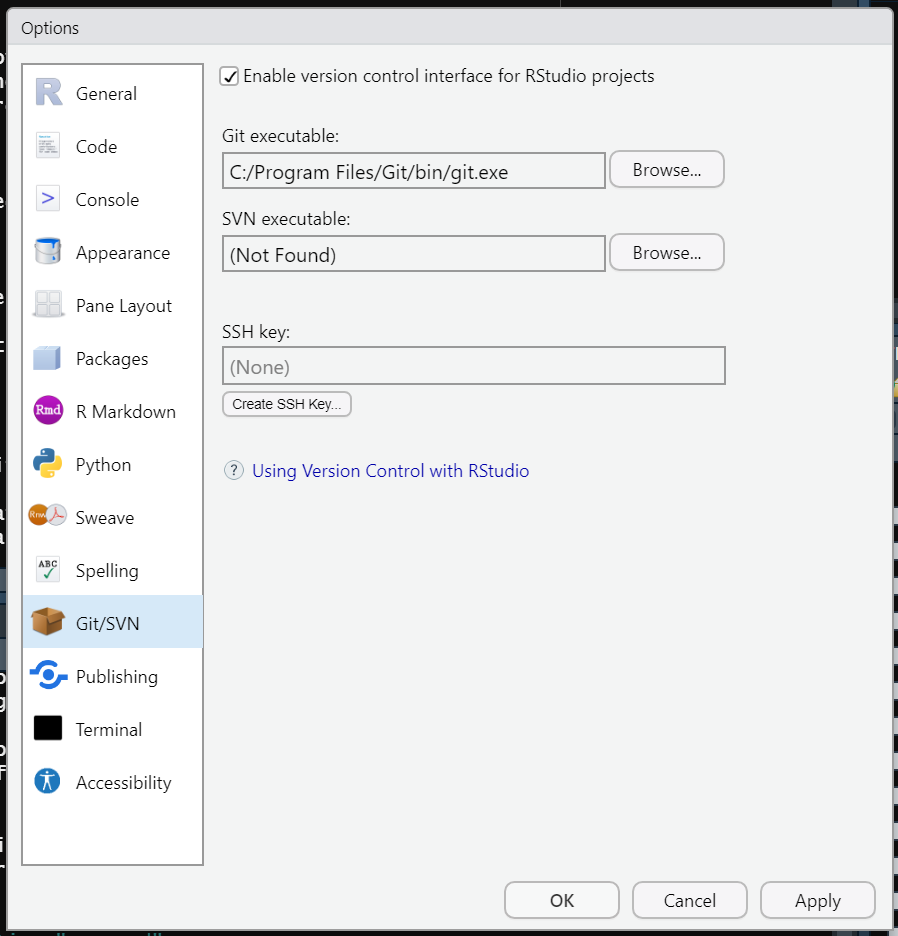
\includegraphics[width=0.64\linewidth]{images/gitdemo/gitdemo-gitRstudio-settings} \caption{Enter the path to your git executable in the git path option box}\label{fig:unnamed-chunk-1}
\end{figure}

Once you open a repository, you'll get an extra panel, named `git', in
the top right pane of R-Studio and you'll also be able to use git in the
`Terminal' tab at the bottom left (in the same place as the R console).

\begin{figure}
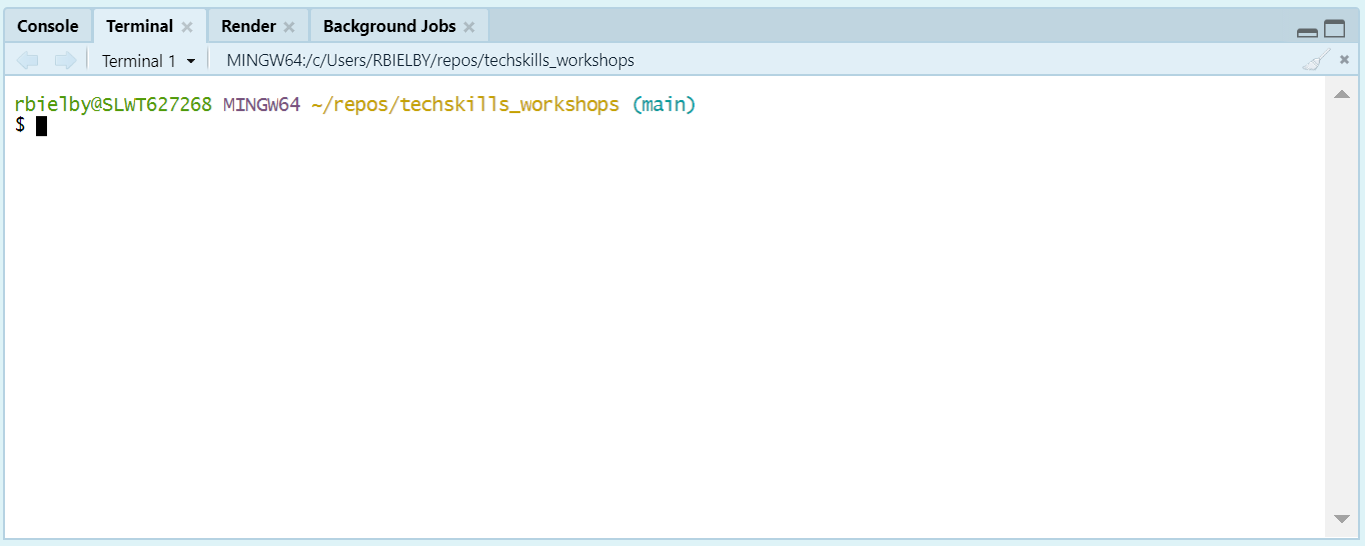
\includegraphics[width=0.56\linewidth]{images/gitdemo/gitdemo-gitRstudio-NewTerminal} \caption{The `git BASH` terminal in R-Studio}\label{fig:unnamed-chunk-2}
\end{figure}

A useful thing here if you want to use git commands in the terminal is
to switch the terminal from the default Windows Command Prompt to
\texttt{git\ BASH}. You can do this in the Terminal tab of R-Studio's
global options - just select \texttt{git\ BASH} from the `New terminal
opens with' pull down menu. Click apply and then select the Terminal tab
(next to the Console tab), click `Terminal 1' and then select `New
terminal' from the drop down menu. You should see something similar to
the terminal screenshot.

\newpage

\hypertarget{setting-up-the-repository}{%
\section{Setting up the repository}\label{setting-up-the-repository}}

\hypertarget{creating-a-new-repository-on-github}{%
\subsection{Creating a new repository on
GitHub}\label{creating-a-new-repository-on-github}}

At this point, we're ready to create a new repository. The context of
this exercise is to create a dashboard, so let's get a head start on
that by using the DfE R-Shiny template.

\begin{figure}
\centering
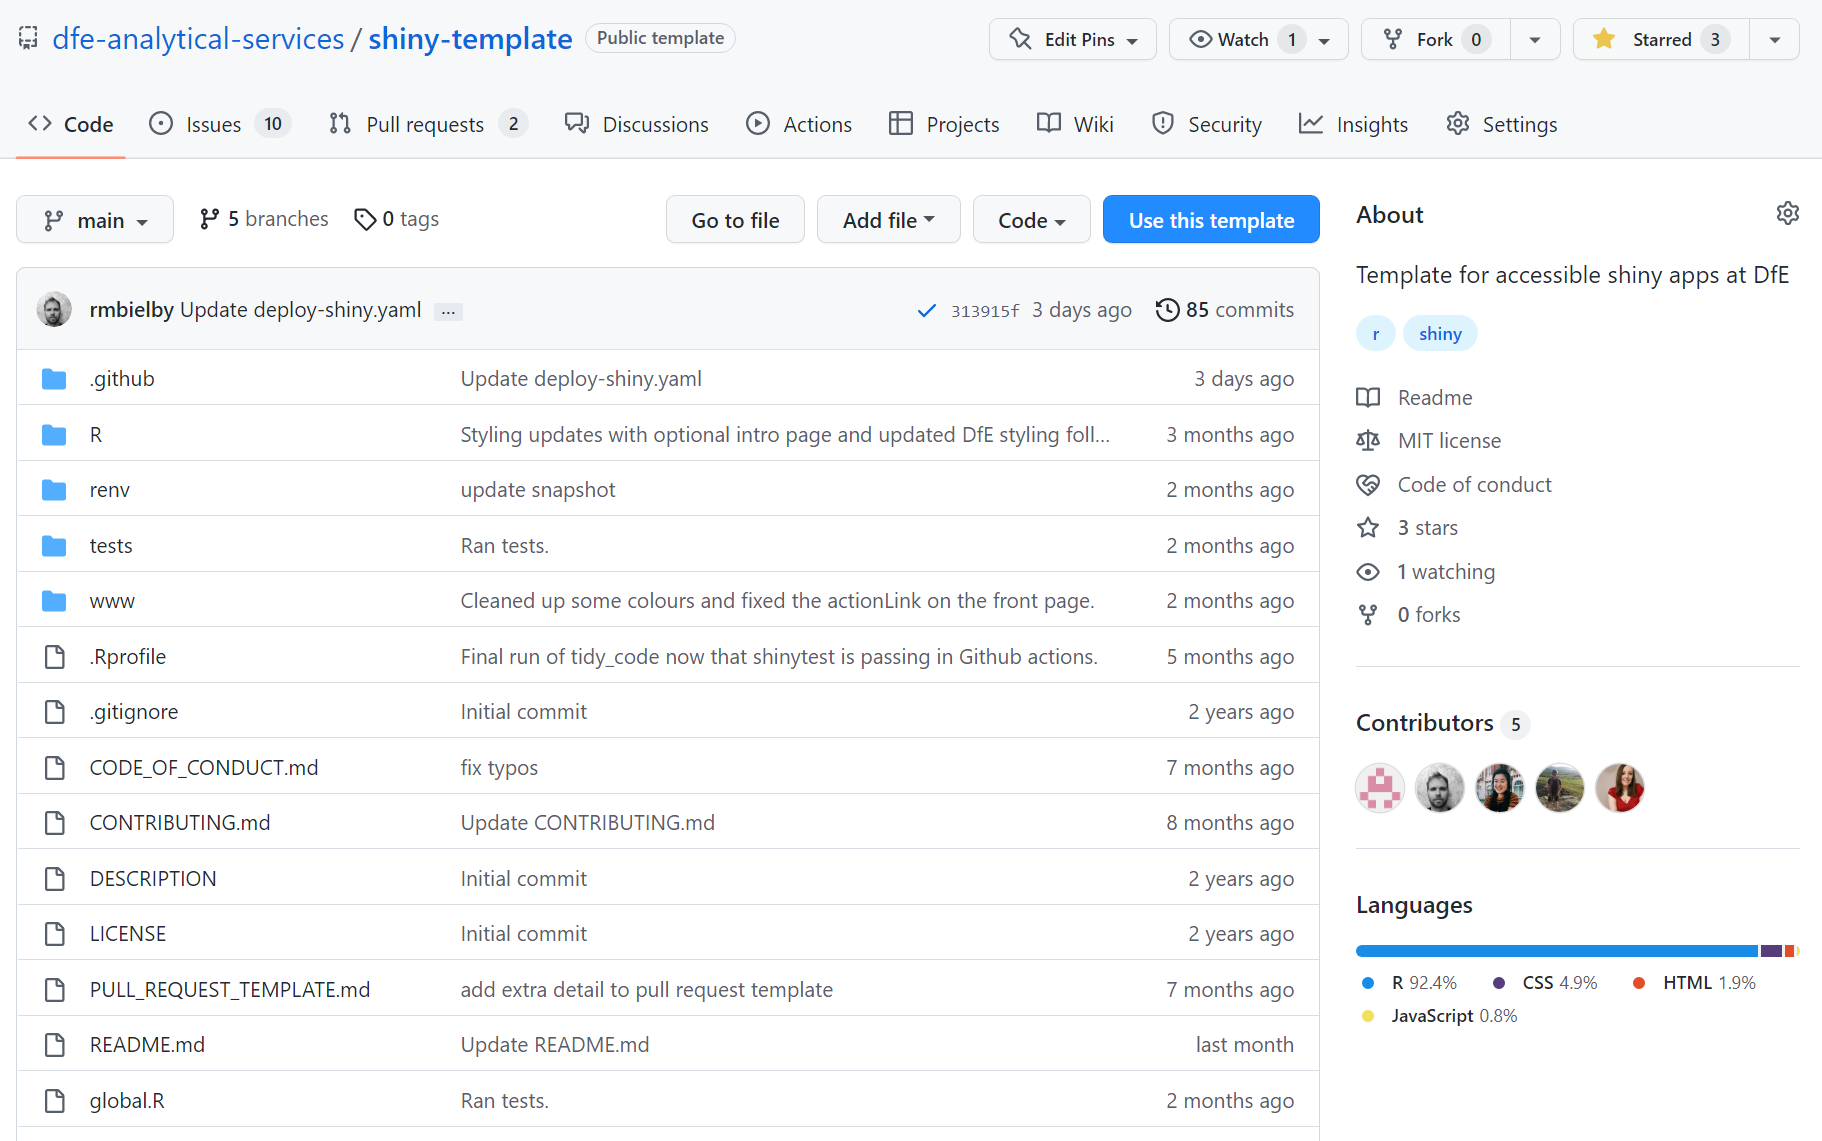
\includegraphics{images/gitdemo/gitdemo-shinydash-template.png}
\caption{Click the use this template button to create the new
repository}
\end{figure}

You can access the template here:

\url{https://github.com/dfe-analytical-services/shiny-template}

On that page, you'll see the main repository page. This contains a menu
bar to navigate the range of GitHub features (e.g.~Code, Issues, Pull
Requests, Discussions, Actions and others); shortcuts to access
different branches within the repository; some top-level summary
information on the repository; a listing of the files and folders in the
repository's root directory; and a markdown render of the repository's
Readme file if one exists.

In the case of our template, you'll also see a button saying use this
repo as a template. At this point, \textbf{one (and only one!)} of your
group should click that button, which will take you to the create
repository page. Here you have the option to create a copy of the
template in your own GitHub area as shown below. Give the new repository
a name and a description and then click ``Create repository from
template''.

\begin{figure}
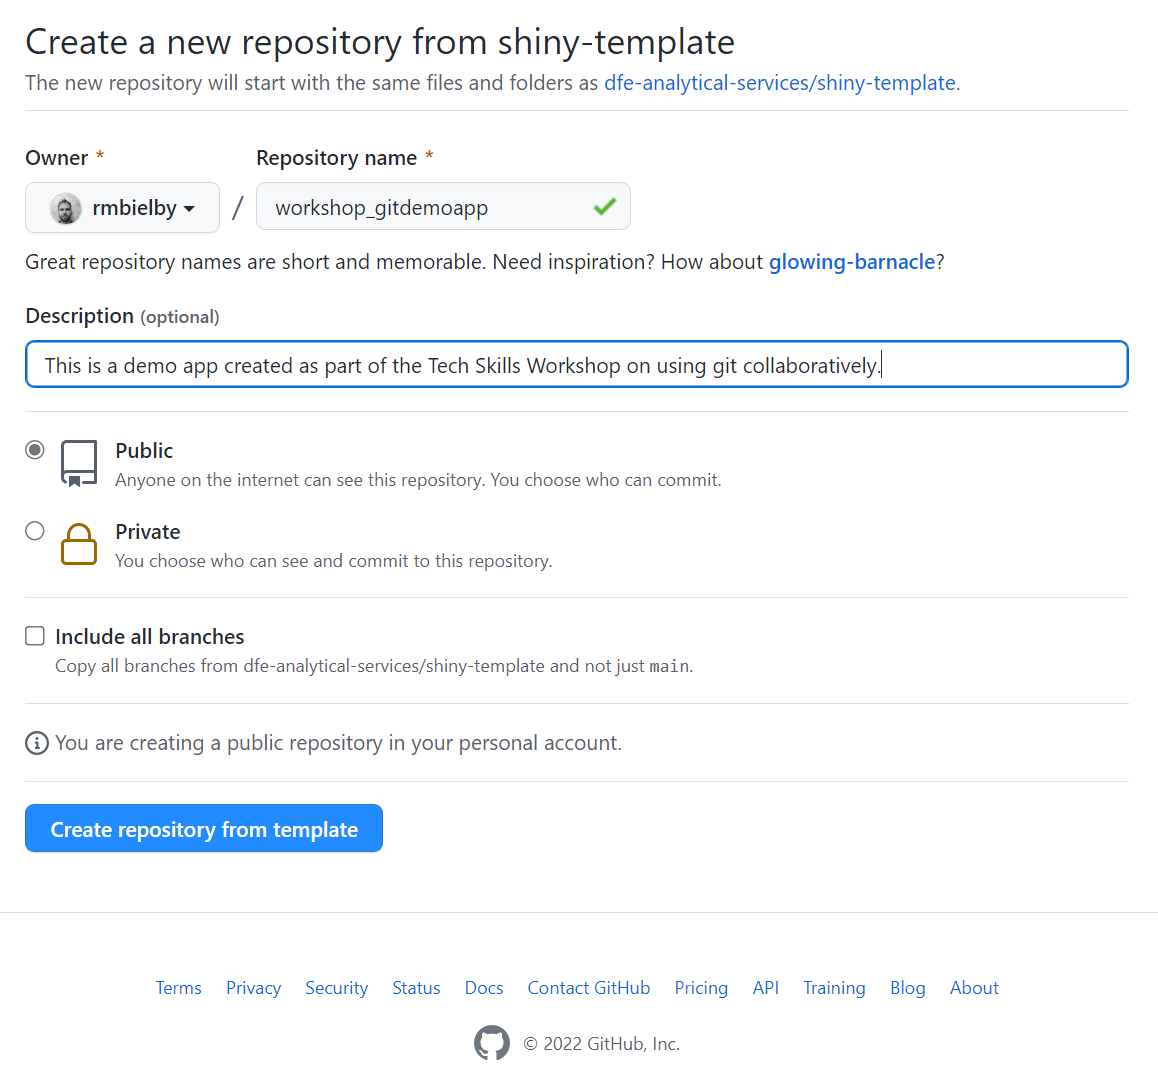
\includegraphics[width=0.72\linewidth]{images/gitdemo/gitdemo-shinydash-newrepofromtemplate} \caption{Put in a name for the new repo and a quick description and then click on Create repository from template}\label{fig:unnamed-chunk-3}
\end{figure}

One of you at least should now have their own repository produced from
this starting template project. We need everyone in your team to be able
to work on this project however, so now you'll need to give access to
your other team members. To do so, navigate to \textbf{Settings} (at the
far right of the menu bar on your repository page) and select
\textbf{Collaborators} on the left hand side. Under \textbf{Manage
access}, add your teammates via either their email addresses or their
GitHub user names.

\hypertarget{cloning-the-repository-to-your-local-machine}{%
\subsection{Cloning the repository to your local
machine}\label{cloning-the-repository-to-your-local-machine}}

Cloning the repository refers to creating a copy of the remote
repository (i.e.~the copy on GitHub or Dev Ops) on the disk on your
local machine (i.e.~your DfE laptop). For an R project, there are two
basic options to choose from for doing this:

\begin{itemize}
\tightlist
\item
  using the R-Studio new project wizard, or
\item
  using \texttt{git\ BASH}.
\end{itemize}

We'd recommend trying the different options across your working group.

\hypertarget{cloning-in-git-bash}{%
\subsubsection{\texorpdfstring{Cloning in
\texttt{git\ BASH}}{Cloning in git BASH}}\label{cloning-in-git-bash}}

You can open up a \texttt{git\ BASH} terminal, by typing
\texttt{git\ BASH} in the Windows search bar and select
\texttt{git\ BASH} when it comes up. With a terminal, you can interact
with it just by typing, similar to working in the R console in RStudio.
First let's make a directory in which to store our repositories:

\begin{verbatim}
    mkdir repos
\end{verbatim}

We can then move into the directory we just created using:

\begin{verbatim}
    cd repos
\end{verbatim}

Now grab the repo url and replace
\texttt{\textless{}repo\_url\textgreater{}} in the next command with the
actual url:

\begin{verbatim}
    git clone <repo_url>
\end{verbatim}

You should get some messages letting you know git is connecting to the
server and cloning the repository and it should look something like the
figure below.

\begin{figure}
\includegraphics[width=0.6\linewidth]{images/gitdemo/gitdemo-terminal_clone} \caption{Cloning a repository in git BASH}\label{fig:unnamed-chunk-4}
\end{figure}

If all went well, you'll now have a complete copy of the repository on
your laptop. To open the repository in RStudio, start up RStudio and
select Open project. In the file explorer window that opens up, type
\texttt{C:\textbackslash{}Users\textbackslash{}} and hit enter (see the
screenshot below) and then open up your home folder.

\begin{figure}
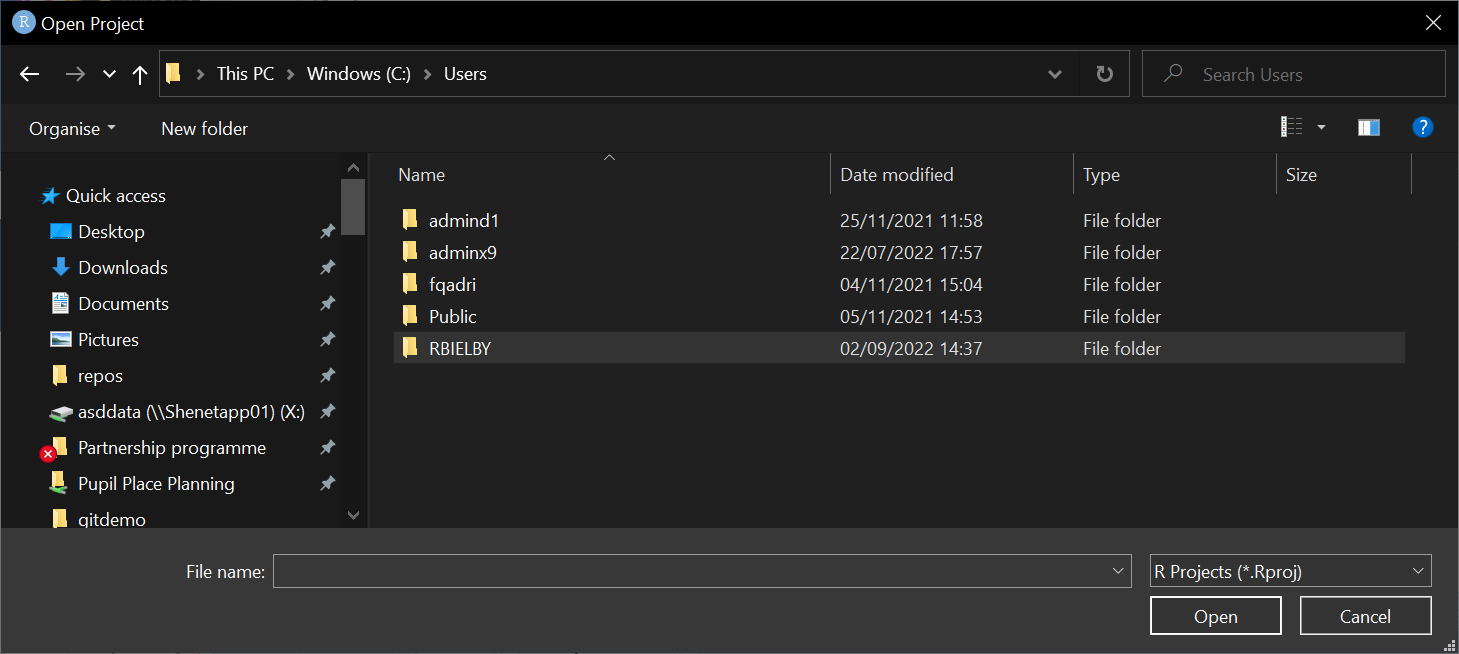
\includegraphics[width=0.6\linewidth]{images/gitdemo/gitdemo-RStudio_OpenProj} \caption{Open a cloned project in RStudio}\label{fig:unnamed-chunk-5}
\end{figure}

Then navigate into \texttt{repos} and the repository folder. The full
path should be something along the lines of:

\begin{quote}
\texttt{This\ PC\ \textgreater{}\ Windows\ (C:)\ \textgreater{}\ Users\ \textgreater{}\ \textless{}USERNAME\textgreater{}\ \textgreater{}\ repos\ \textgreater{}\ \textless{}REPONAME\textgreater{}}
\end{quote}

Select the R project file and select open.

\begin{figure}
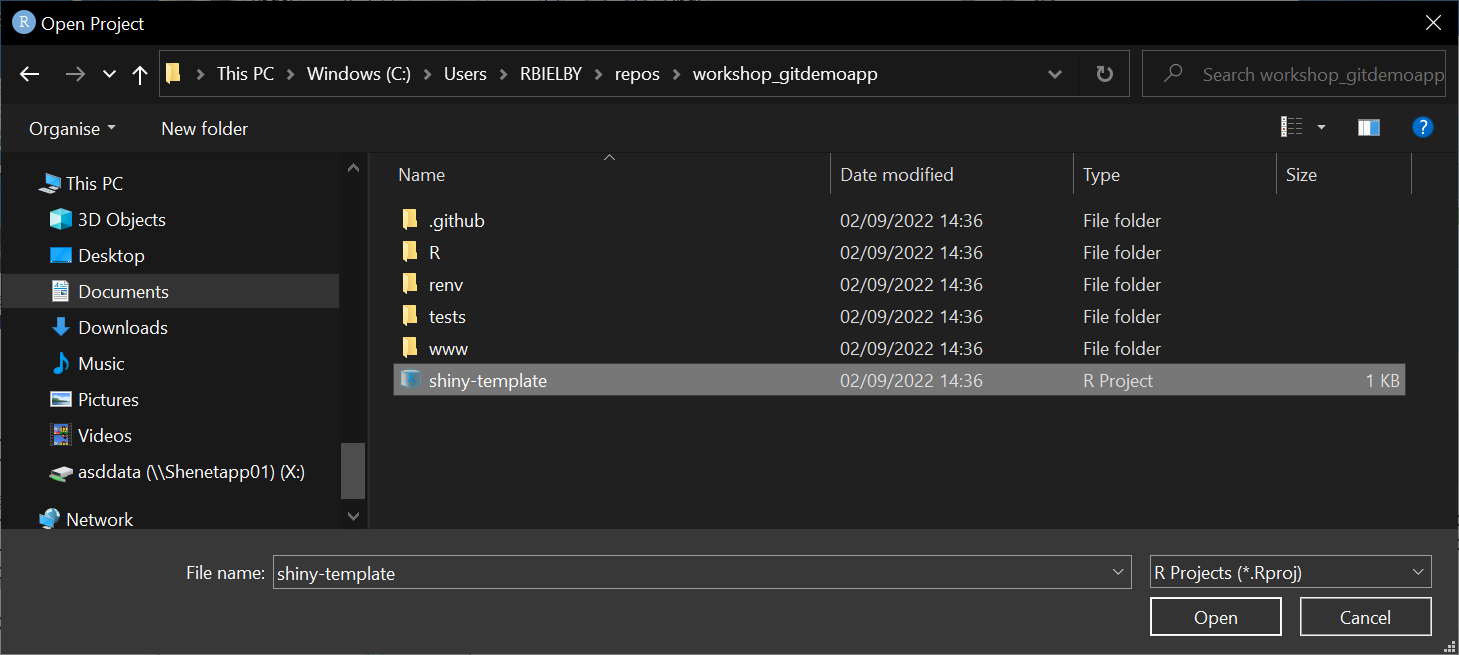
\includegraphics[width=0.6\linewidth]{images/gitdemo/gitdemo-RStudio_OpenProj_fullpath} \caption{Open a cloned project in RStudio}\label{fig:unnamed-chunk-6}
\end{figure}

\hypertarget{cloning-using-the-rstudio-wizard}{%
\subsubsection{Cloning using the RStudio
wizard}\label{cloning-using-the-rstudio-wizard}}

If that looks like a bit too much text based effort, RStudio offers a
way to clone a repository with it's New project wizard. To do this
navigate the menu bar to \textbf{File \textgreater{} New
Project\ldots{}}, select \textbf{Version Control} and then Git. This
opens up a dialogue box to enter the repository url and select where to
save it. As with the git BASH version, copy and paste your remote repo
URL here and set a directory where you want it saved on your laptop.

\begin{figure}
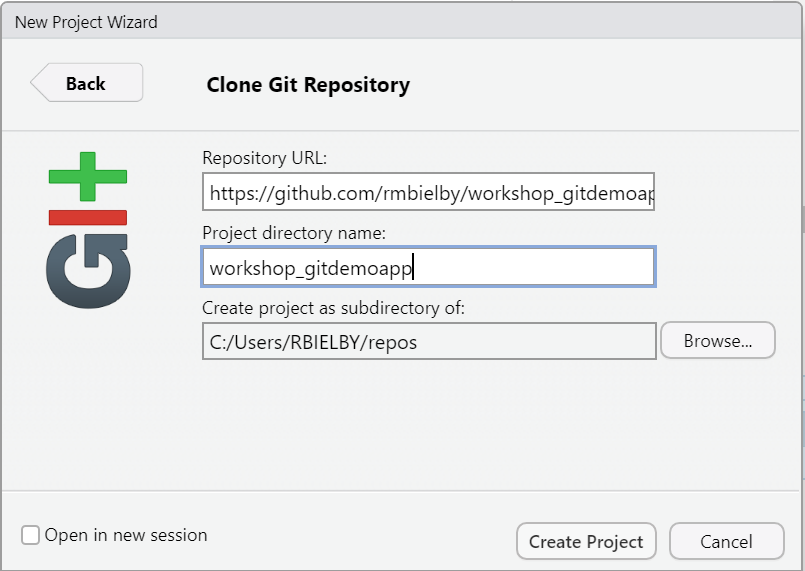
\includegraphics[width=0.6\linewidth]{images/gitdemo/gitdemo-RStudio_OpenProj_wizard} \caption{Clone a project using the RStudio git wizard}\label{fig:unnamed-chunk-7}
\end{figure}

\hypertarget{a-note-on-local-repository-clones-and-onedrive}{%
\paragraph{A note on local repository clones and
OneDrive}\label{a-note-on-local-repository-clones-and-onedrive}}

\begin{quote}
Note that saving a repository within your OneDrive folder structure can
cause some awkward issues. If you use git to perform version control on
a repository saved within a OneDrive folder, you may start receiving
warning messages that large numbers of files have been removed from
OneDrive. In addtion, it can put a heavy burden on your internet
connection as OneDrive tries to keep up with changes to the files
managed by git. Best practice therefore is to store your repositories
somewhere outside your OneDrive file structure. We recommend creating a
\texttt{repos} directory within your base User directory
(i.e.~\texttt{C:\textbackslash{}Users\textbackslash{}\textless{}USERNAME\textgreater{}\textbackslash{}repos\textbackslash{}}.
Windows sometimes tries to make it awkward for you to navigate to places
on your laptop outside of the OneDrive folders, so a useful tip is to
add your \texttt{repos} folder to your Quick access list in File
Explorer.
\end{quote}

\hypertarget{controlling-packages-with-renv}{%
\subsection{Controlling packages with
renv}\label{controlling-packages-with-renv}}

Now that you've each got a clone of the repository, it's useful to
understand a little bit about environment control. Using R as the
specific example, any app or pipeline that you develop will have
packages that it depends on. If someone wants to use your code, they
need to know what packages are involved, whilst it can also be helpful
for them to be able to use the same versions of those packages in order
to recreate exactly what you intended the code to be able to do.

To manage this, we can use an R package called \texttt{renv}. This
manages the R environment for you, helping you keep track of your
repositories required R packages and their versions. In a brand new
empty project, you'd initiate \texttt{renv} with the command
\texttt{renv::init()}. In this case, the template already has
\texttt{renv} initiated. So instead we can tell renv to check the
necessary packages and install them for us. You can do this by entering
the following command in the R console:

\begin{verbatim}
    renv::restore()
\end{verbatim}

This should go through \texttt{renv}'s list of the required packages and
install them all in one go (note that you'll need to be connected to the
internet for it to retrieve any packages that aren't already installed).
Once you've done this, the contents of the repository should run as
intended. If at some point you install an extra package for the
repository, you can add this to \texttt{renv}'s package list by entering
the command \texttt{renv::snapshot()} into the R console.

\hypertarget{running-the-dashboard-template-locally}{%
\subsection{Running the dashboard template
locally}\label{running-the-dashboard-template-locally}}

Once you've cloned the package and run \texttt{renv::restore}, you
should then be able to run the Shiny dashboard template. To do this,
either a) enter \texttt{shiny::runApp()} in the R console or b) open up
the file \textbf{ui.R} and then click \textbf{run App} to the top right
of the editor pane. The dashboard should then load either in an RStudio
window or in your default web browser (depending on your chosen settings
in RStudio).

\begin{figure}
\centering
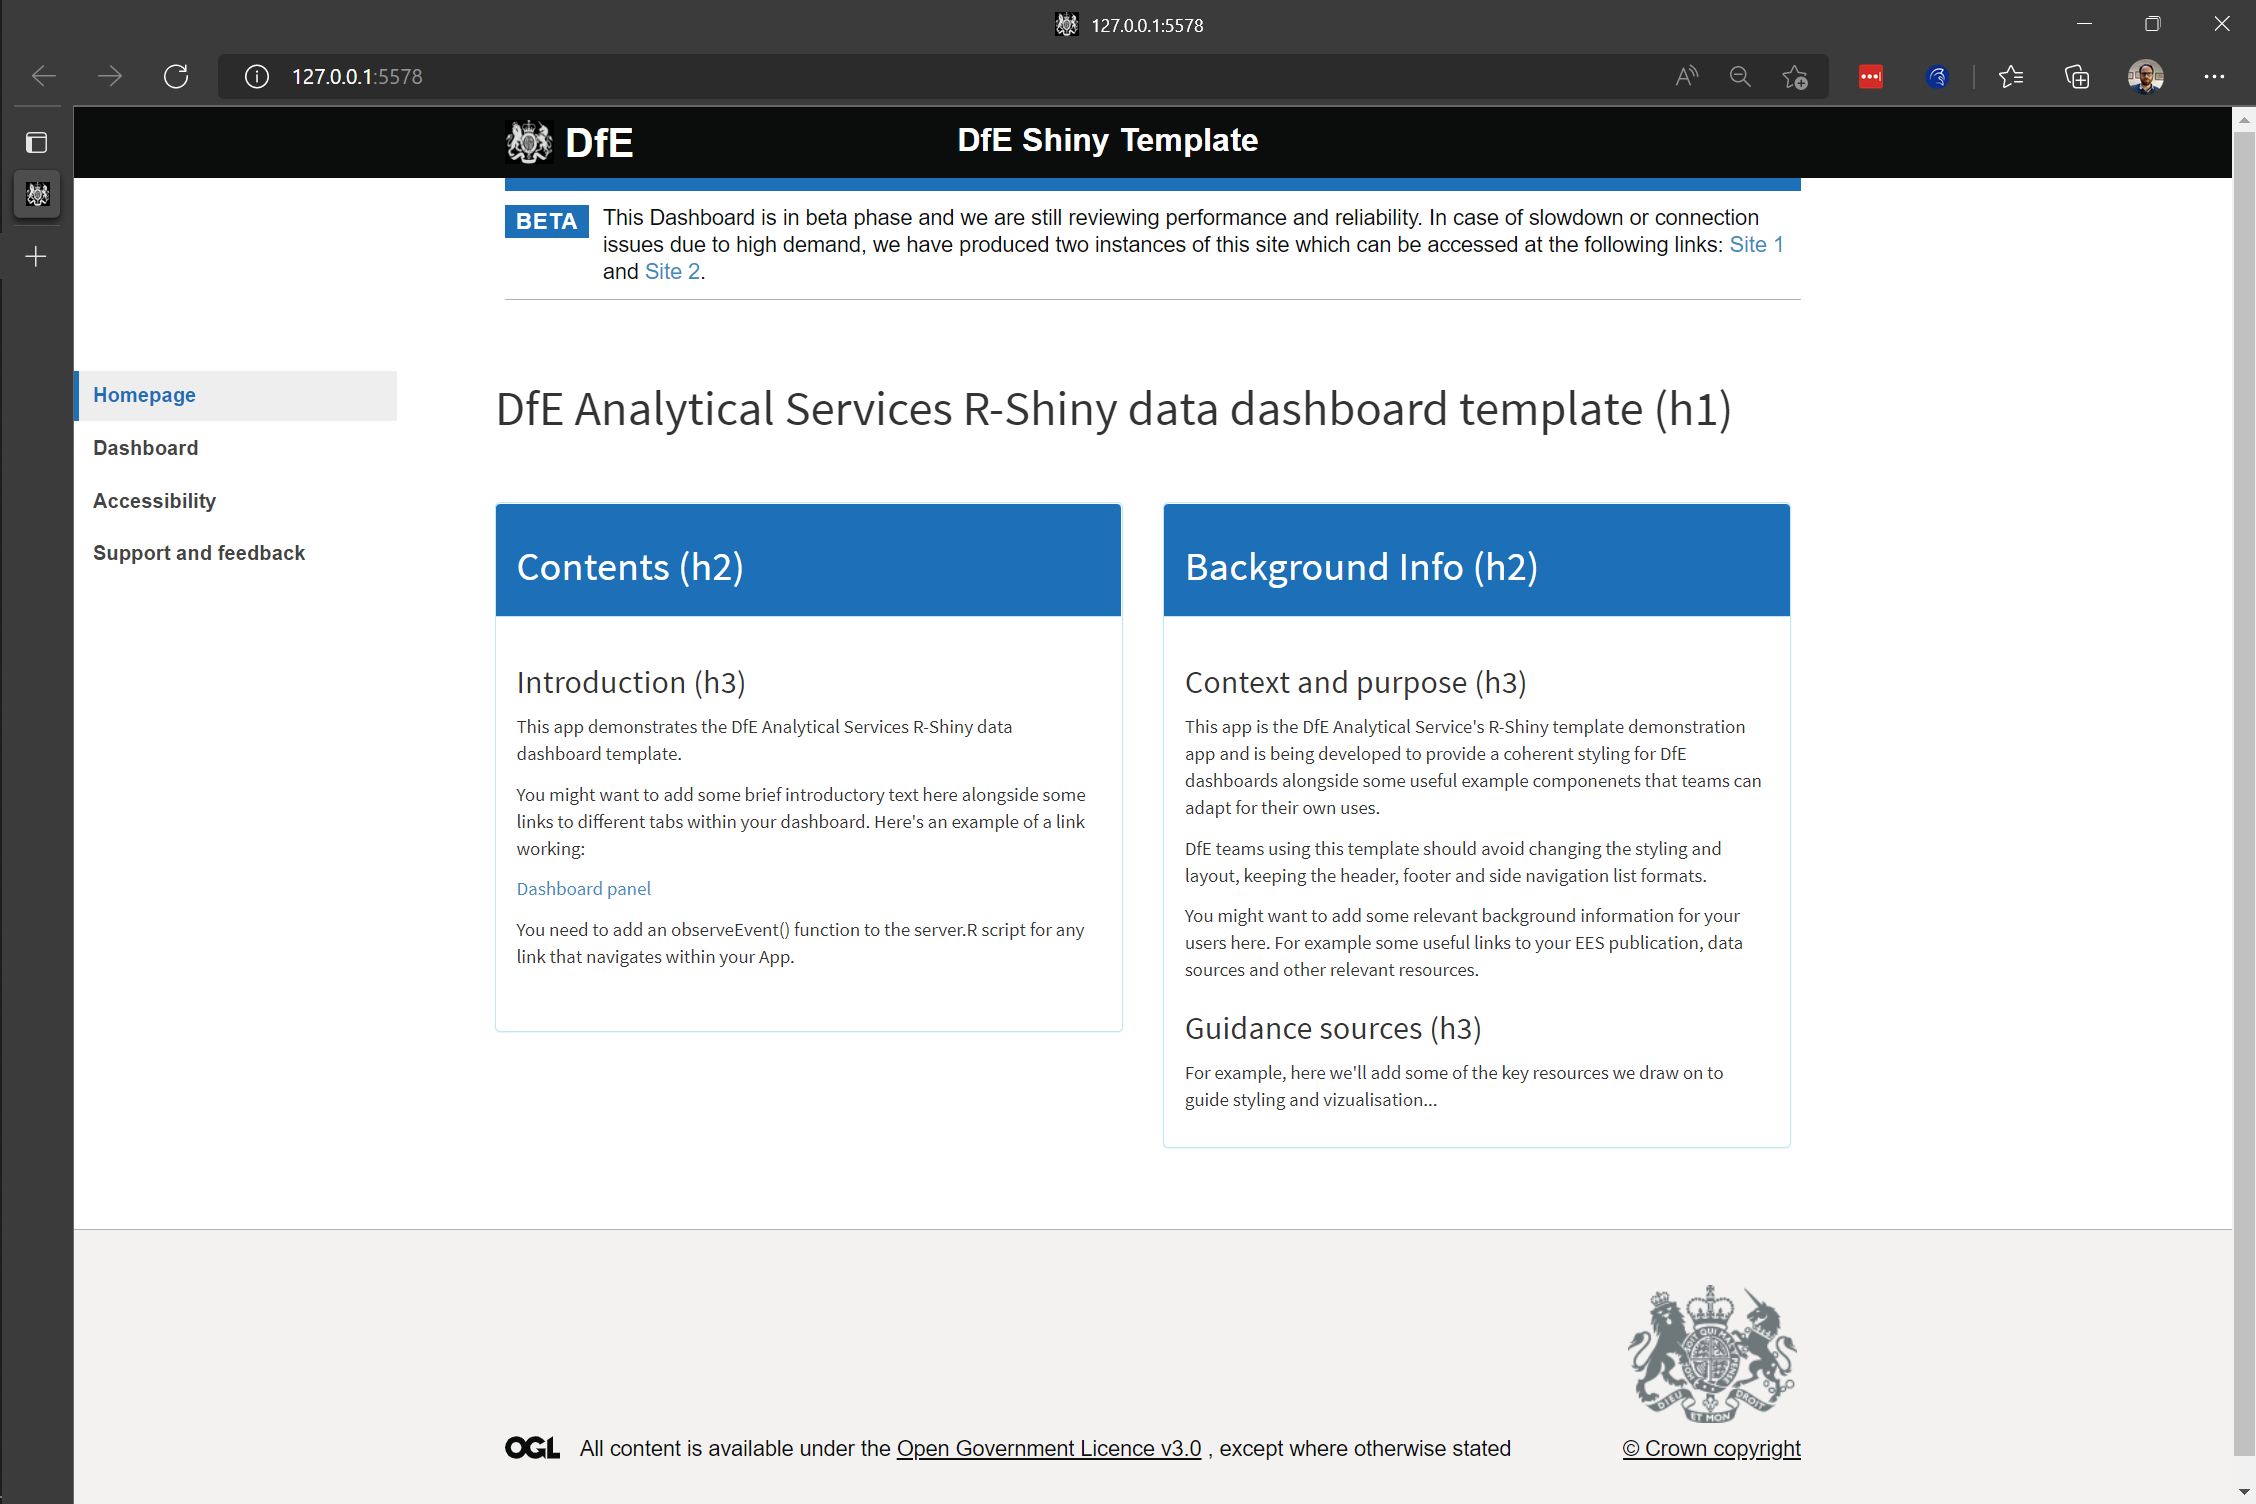
\includegraphics{images/gitdemo/gitdemo-ShinyAppTemplate.PNG}
\caption{The DfE R-Shiny template loaded locally from RStudio}
\end{figure}

Although this workshop is primariy a chance to practice using git,
you'll need a little understanding of the components of an R-Shiny app
as well. A single app generally consists of 3 key scripts:
\emph{global.R}, \emph{ui.R} and \emph{server.R}. Each of these fulfills
a specific purpose as follows:

\begin{itemize}
\tightlist
\item
  \emph{global.R}: contains variables and functions required by the rest
  of the app (e.g.~reading in data, connecting to a database);
\item
  \emph{ui.R}: contains code to create the app's user interface
  (e.g.~arranging the layout, placement of charts, tables and text);
\item
  \emph{server.R}: contains the functions that make the app responsive
  (e.g.~rendering tables and charts and updating dynamic text and input
  fields).
\end{itemize}

We'll explain more as needed, but for now that should give you the basic
overview.

\hypertarget{summary}{%
\subsection{Summary}\label{summary}}

In this section, we've covered creating a repository via a template on
GitHub, cloning it to your local drive (using both the BASH terminal and
the RStudio wizard) and getting the necessary packages installed in one
go with \texttt{renv::restore()} via the R console.

In the next section, we'll cover some of the basics of using git to log
changes to your code and sync them between the remote repo and local
copies.

\newpage

\hypertarget{basics-of-git}{%
\section{Basics of git}\label{basics-of-git}}

We'll now take a look at updating repositories with your working. To do
so, we'll follow some example first steps you might take with developing
the template dashboard app to use your own data. The steps we'll follow
will be to create a new branch, add the data in, commit it to the github
log and then push it to the remote (GitHub) repository.

\hypertarget{the-git-log}{%
\subsection{The git log}\label{the-git-log}}

In order to move quickly between different versions of files and code,
git is built around indexing and a log file that track the changes in a
repository. To view the log of any repository, we can simply go into
that repository and run the command \texttt{git\ log} from the BASH
terminal. For example, if you run it in the repository you've created
from the template, you'll get something along the lines of the
following:

\begin{center}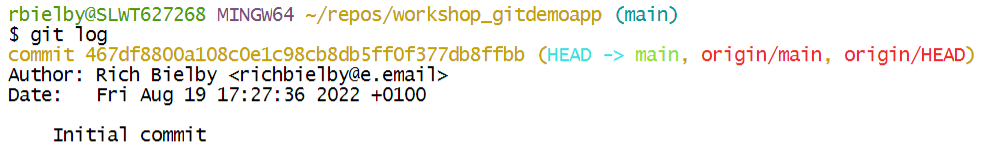
\includegraphics[width=0.8\linewidth]{images/gitdemo/gitdemo-gitlog-1} \end{center}

The log shows all ``commits'' that have been made to the repository.
We'll go into making commits in the next section.

\hypertarget{adding-commiting-and-pushing}{%
\subsection{Adding, commiting and
pushing}\label{adding-commiting-and-pushing}}

To adapt the existing template, we want to add some new data. There
should be a data folder in the repository already, so all we need to do
is grab some data and save it there. For this workshop, we'll use a file
from a publication on Explore Education Statistics.

\emph{Again, for this section, just one of your group should run through
the following steps:}

Go to
\href{https://explore-education-statistics.service.gov.uk/data-catalogue/progression-to-higher-education-or-training/2019-20}{the
progression to higher education or training data catalogue} and download
the \textbf{Progression to higher education and training - Local
authority level (csv, 4 Mb)} file, extract the data csv file
(\emph{l4\_tidy\_2020\_all\_la.csv}) and save it into the repo's data
folder.

Now to add this to the git tracking: run the following commands:

\begin{verbatim}
  git add .
\end{verbatim}

This searches the repo for any files that have been modified since the
last commit and creates a log of the changes.

\begin{verbatim}
  git commit -m "Added data file into repository."
\end{verbatim}

This adds an entry on to the log, updating it with the file changes that
you've just made. Note that the text after the \texttt{-m} is a comment
used to describe the changes to make it easier for someone looking back
from the log to see what changes have happened. Those are the two key
steps for tracking changes to the files and folders in your repository.
Say we decide we're not happy with the data filename, maybe we think the
filename should be more informative for users. We'd now change the
filename as normal (e.g.~to \emph{progress\_he\_la\_2020.csv} using File
Explorer), and then run the commands

\begin{verbatim}
   git add data/progress_he_la_2020.csv
\end{verbatim}

and

\begin{verbatim}
   git commit -m "Made data filename more informative."
\end{verbatim}

Note that in this instance, we're adding just a single specific file (by
naming the file in the \texttt{git\ add} comand), rather than asking git
to check the whole repo for any updated files (i.e.~by using
\texttt{git\ add\ .}). We've also updated the commit message to be
informative about the changes that we've made. If we now run
\texttt{git\ log} again, we get something along the lines of:

\begin{center}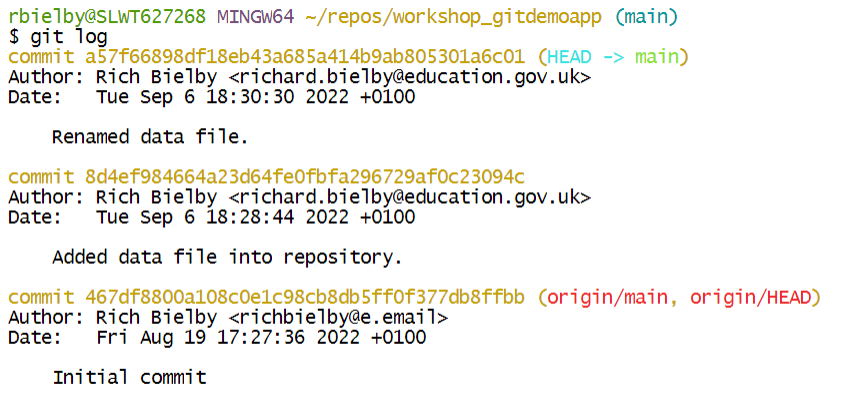
\includegraphics[width=0.8\linewidth]{images/gitdemo/gitdemo-gitlog-2} \end{center}

Here we can see, in reverse order, the commits that have been made, who
made them, when they made them, and the messages that have been recorded
with them.

Finally, it's important to note that what we've done so far is only
being applied to the local copy of the repository (i.e.~the copy on your
laptop). To apply your changes to the remote repository (i.e.~on GitHub
or Dev Ops), you need to ``push'' the changes. This can be done a couple
of different ways: a) in the terminal type \texttt{git\ push} or b) on
the toolbar in the git tab in RStudio press the green up button! Once
you've done this, open up a browser and go to your remote repository on
GitHub and you should now see the data file stored there.

\hypertarget{pulling-from-the-remote-repository}{%
\subsection{Pulling from the remote
repository}\label{pulling-from-the-remote-repository}}

Now that you've made changes, the rest of your team can update their own
local copies of the repository with your updates by pulling from the
remote. Similarly to pushing, they can do this by either a) typing
\texttt{git\ push} in the BASH terminal or b) pressing the down arrow in
the toolbar of the git tab in RStudio.

\hypertarget{summary-of-git-basics}{%
\subsection{Summary of git basics}\label{summary-of-git-basics}}

We've quickly tried out a quick cycle of adding and committing, which is
used to log changes into the local repository and then we've pushed and
pulled to and from the remote repository and local copies on different
laptops. The table below gives a summary of the relevant commands in the
BASH terminal and the corresponding buttons in the RStudio git panel.

\begin{longtable}[]{@{}
  >{\raggedright\arraybackslash}p{(\columnwidth - 4\tabcolsep) * \real{0.0968}}
  >{\raggedright\arraybackslash}p{(\columnwidth - 4\tabcolsep) * \real{0.3763}}
  >{\raggedright\arraybackslash}p{(\columnwidth - 4\tabcolsep) * \real{0.5269}}@{}}
\toprule()
\begin{minipage}[b]{\linewidth}\raggedright
Process
\end{minipage} & \begin{minipage}[b]{\linewidth}\raggedright
git BASH
\end{minipage} & \begin{minipage}[b]{\linewidth}\raggedright
RStudio git panel
\end{minipage} \\
\midrule()
\endhead
Add & \texttt{git\ add\ .} & Stage using tickbox next to each modified
file. \\
Commit & \texttt{git\ commit\ -m\ "Commit\ message."} & ``Commit''
button in toolbar. \\
Push & \texttt{git\ push} & Green up arrown in toolbar. \\
Pull & \texttt{git\ pull} & Blue down arrow in toolbar. \\
View the log & \texttt{git\ log} & Clock icon in toolbar. \\
\bottomrule()
\end{longtable}

\newpage

\hypertarget{working-collaboratively-with-git}{%
\section{Working collaboratively with
git}\label{working-collaboratively-with-git}}

Git only really makes proper sense once multiple people start working on
a project collaboratively. Solo working, git is useful for version
control and syncing your work to a remote repository site like Dev Ops
and GitHub, but may not feel like it offers all that much more beyond
that. Once we start working collaboratively however, the benefits of
using git (alongside GitHub or Dev Ops) become more apparent. We'll now
look further into this with some worked examples.

\hypertarget{branches-and-splitting-tasks}{%
\subsection{Branches and splitting
tasks}\label{branches-and-splitting-tasks}}

\hypertarget{task-management}{%
\subsubsection{Task management}\label{task-management}}

One useful management tool that we can use from GitHub is the Issues
tab. Here we can create individual tasks, assign them to team member and
then create new \textbf{branches} from those tasks. You can think of
\textbf{branches} as self contained copies of the repository that can
contain complementary or conflicting differences with all other
\textbf{branches} in the repository. These allow you to work on
different multiple tasks on your code independently of any other changes
you might be making. Bringing these different \textbf{branches} or tasks
together is then managed using \textbf{merges} or \textbf{pull requests}
(PRs).

We'll demonstrate this by performing 3 related tasks on 3 different
branches. Each task should be done by only one of your group, so split
the following 3 tasks between your group and each follow the relevant
instructions in the subsections below:

\begin{itemize}
\tightlist
\item
  1a) Reading in the data
\item
  1b) Updating references in the server script and the user interface
\item
  1c) Creating a chart
\end{itemize}

Once you've decided who's doing what, each of you should jump to the
relevant section below. And remember that you're not working in
independent silos here, what you do can impact what other people are
doing so communication needs to happen along the way.

\hypertarget{task-1a---reading-in-the-data}{%
\paragraph{Task 1a - Reading in the
data}\label{task-1a---reading-in-the-data}}

This task underpins the next two. You need to read in the data file that
we've already downloaded. Start by creating a new branch: go to the BASH
terminal, and type:

\begin{verbatim}
  git checkout -b featReadData
\end{verbatim}

This creates and moves you into a new branch called featReadData.
Anything you do here has no affect on the contents of the main branch
until you explicitly tell git to merge your changes. Note that this only
creates the branch in your local copy of the repository, for it to be
added to the remote, you'll need to push:

\begin{verbatim}
  git push --set-upstream origin featReadData
\end{verbatim}

Note that if you only enter \texttt{git\ push} without the
\texttt{set-upstream} flag, git will suggest the full command for you.

Now to write the code in this branch that's going to read in the data.
We'll read it in to a data frame and the first task is to choose a name
for the data frame and let the rest of the team know, as they'll need
that info (in the example below, we're calling it
\texttt{dfProgressHE}). If you've got the R expertise to do this
already, then feel free to go for it, otherwise just follow the
following steps below.

Open up the script \texttt{R/read\_data.R} and change the code from:

\begin{verbatim}
  read_revenue_data <- function(file){
    dfRevenue <- read.csv(file)
    colnames(dfRevenue)[1] <- "time_period"
    dfRevenue <- dfRevenue %>% 
      mutate(year = as.numeric(paste0("20",substr(format(time_period),5,6))),
      area_name=case_when(geographic_level=='National' ~ country_name,
                       geographic_level=='Regional' ~ region_name,
                       TRUE ~ la_name))
    return(dfRevenue)
  }
\end{verbatim}

to:

\begin{verbatim}
  funcReadData <- function(file){
    dfData <- read.csv(file)
    dfData <- dfData %>% 
      mutate(year = as.numeric(paste0("20",substr(format(time_period),5,6)))) %>%
      filter(geographic_level != "Parliamentary constituency",
             characteristic_group=='Total',
             institution_type=='Total') %>%
      mutate(area_name=case_when(geographic_level=='National' ~ country_name,
                          geographic_level=='Regional' ~ region_name,
                          TRUE ~ la_name))
    return(dfData)
  }
\end{verbatim}

You've made a substantive change, so let's run a quick add, commit and
push in the BASH terminal:

\begin{verbatim}
  git add .
  git commit -m "Added function to read data in data."
  git push
\end{verbatim}

We've made a function to read in the data, but we're not running that
function anywhere. So now open up \emph{global.R} and change the line:

\begin{verbatim}
  dfRevBal <- read_revenue_data()
\end{verbatim}

to the following:

\begin{verbatim}
  dfProgressHE <- funcReadData('data/progress_he_la_2020.csv')
\end{verbatim}

Then change the following lines from:

\begin{verbatim}
  choicesAreas <- dfAreas %>%
    filter(geographic_level == "National") %>%
    select(geographic_level, area_name = country_name) %>%
    rbind(dfAreas %>% filter(geographic_level == "Regional") %>% 
    select(geographic_level, area_name = region_name)) %>%
    rbind(choicesLAs)
  choicesYears <- unique(dfRevBal$time_period)
  choicesPhase <- unique(dfRevBal$school_phase)
\end{verbatim}

to:

\begin{verbatim}
  choicesAreas <- dfAreas %>%
    filter(geographic_level == "Regional") %>% 
    select(geographic_level, area_name = region_name) %>%
    rbind(choicesLAs)
  choicesYears <- unique(dfProgressHE$time_period)
  choicesPhase <- unique(dfProgressHE$data_type)
\end{verbatim}

Give it a test, by sourcing \emph{global.R} in the R console:

\begin{verbatim}
   source("global.R")
\end{verbatim}

And then have a check of the contents of \texttt{dfProgressHE} (e.g.~by
typing \texttt{dfProgressHE} in the R console). It's also worth having a
look through the contents of the \texttt{choicesAreas},
\texttt{choicesYear} and \texttt{choicesPhase} variables to get an idea
of what they contain.

Once you're happy, then run another
\texttt{add}/\texttt{commit}/\texttt{push} cycle and flag to your team
that you've finished the code to read in the data.

\hypertarget{task-1b---updating-the-user-interface-inputs}{%
\paragraph{Task 1b - Updating the user-interface
inputs}\label{task-1b---updating-the-user-interface-inputs}}

Whilst task 1a is updating the data that's been read in, this task aims
to tweak some of the code to make sure the dashboard still works. As
we're no longer working with the same data, we've changed the name of
the data frame holding it and as well some of the column names will be
different.

In this task, we'll create a new branch using GitHub. Open up the
repository on GitHub in your web browser and select the Issues tab. You
should see something similar to shown below.

\begin{figure}

{\centering 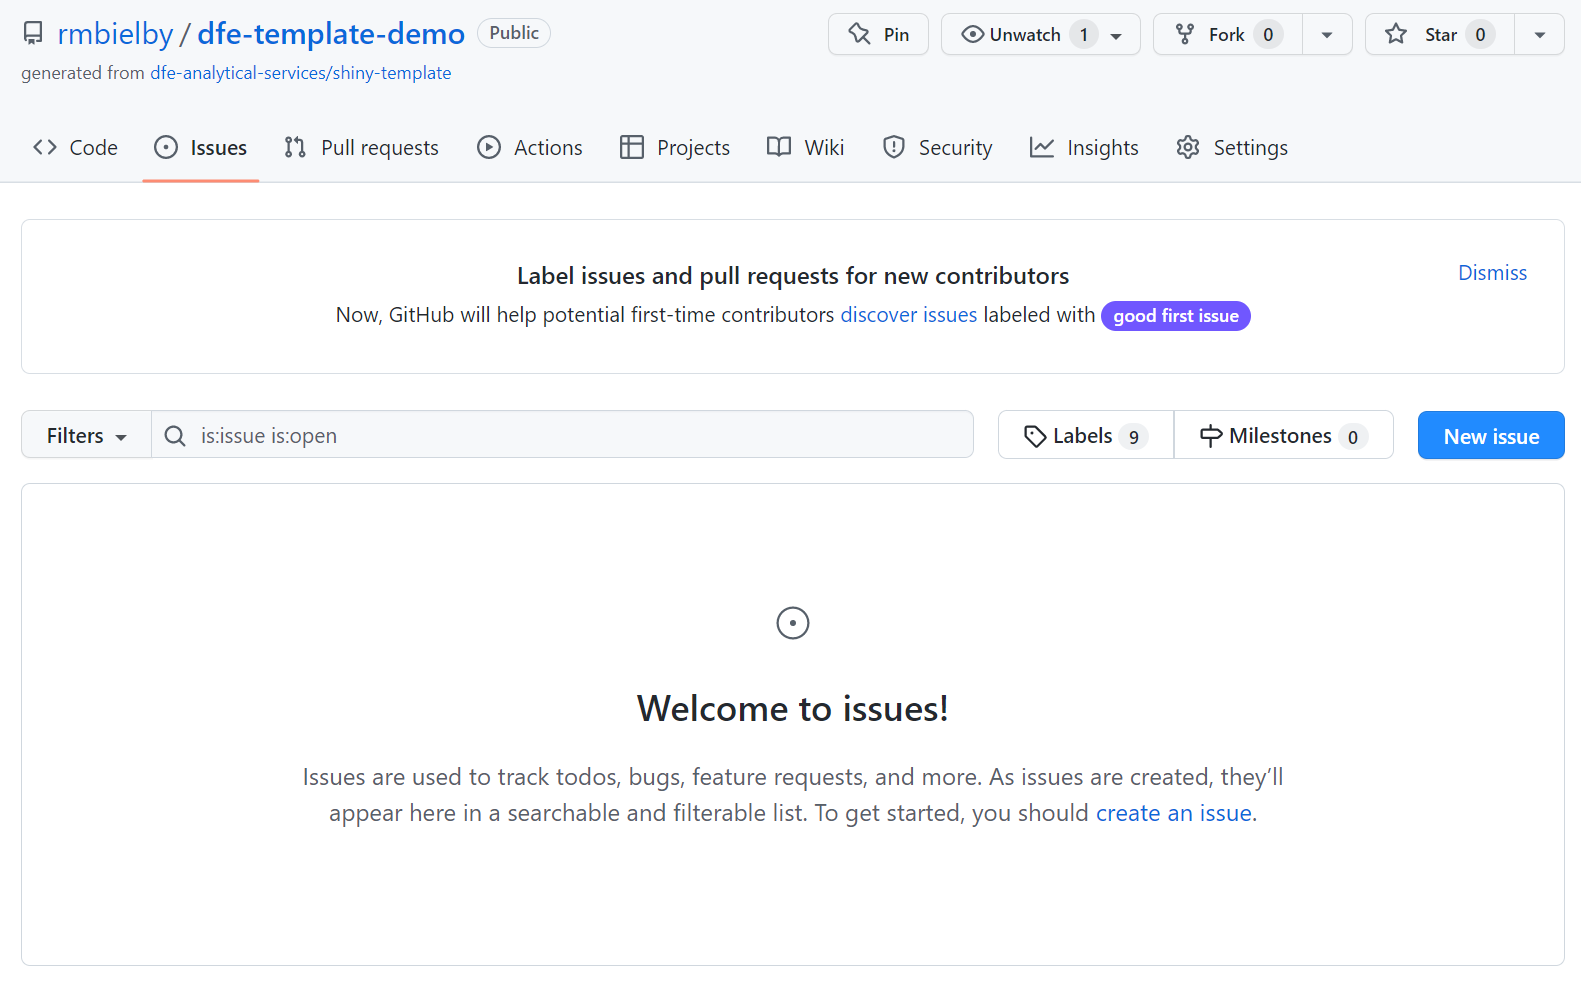
\includegraphics[width=0.92\linewidth]{images/gitdemo/gitdemo-GitHub-Issues} 

}

\caption{The Issues panel in GitHub. This can be used to keep track of jobs that need doing on a repository and create new branches linked to individual jobs.}\label{fig:unnamed-chunk-10}
\end{figure}

On the issues tab, select \emph{New issue} and then click \textbf{Get
started} alongside \textbf{Feature request}. This will open a new issue
panel, with boxes to put in some details about the feature being
requested. Let's put in a title of \emph{``Update inputs for new
data''}. You'll see some handy guidance on what information to enter for
an issue. Have a quick read of this, but then for brevity here, let's
ignore it and put in a short description along the lines of ``The data
file being read in has been updated and the inputs needed updating to
match the column headers etc.''. You've got options to add assign this
task and add labels, link to projects and milestones. We don't need much
of that, but maybe add yourself as the assignee. When you're ready,
click \textbf{Submit new issue}.

After you've done so, you'll see you now have the option in the right
hand side panel to create a new branch linked to this issue. Select that
and choose to check out the branch locally as the next option. Once
you've confirmed you'll get some code to use to checkout the branch
locally, which you can copy and use in the terminal in RStudio. It
should look something like this:

\begin{verbatim}
  git fetch origin
  git checkout 1-update-inputs-for-new-data
\end{verbatim}

Run that in the \texttt{BASH} terminal in RStudio and you'll have your
new branch ready to go.

\begin{figure}

{\centering 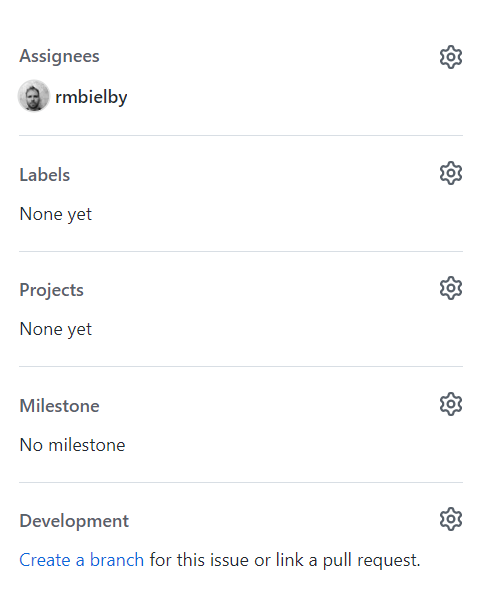
\includegraphics[width=0.64\linewidth]{images/gitdemo/gitdemo-GitHub-Issues-NewBranch} 

}

\caption{Once you've created an Issue on GitHub, you can create a new branch from the GitHub webpage and then fetch it to work on locally on your laptop.}\label{fig:unnamed-chunk-11}
\end{figure}

So we've got a few small changes just to update here given the changes
to the input data. Whoever's performing Task 1a, should be updating the
data frame containing the new input data to be called
\texttt{dfProgressHE} to reflect the different data that's being read
in. The main changes that are needed are in the \emph{server.R} and
\emph{R/dashboard\_panels.R}.

Open up \emph{server.R} and replace any instances of \texttt{dfRevBal}
with \texttt{dfProgressHE} and any instances of \texttt{school\_phase}
with \texttt{data\_type} (which references a specific column within the
data frame).

Then in \emph{R/dashboard\_panels.R}, update the titles of the input
boxes from:

\begin{verbatim}
  selectizeInput("selectPhase",
        "Select a school phase",
        choices = choicesPhase
\end{verbatim}

to:

\begin{verbatim}
  selectizeInput("selectPhase",
        "Select an indicator",
        choices = choicesPhase
\end{verbatim}

And that should be it for this task. All that's left is to commit and
push your changes. If you've got a preferred way already to perform
commits, then go for it. If not then let's use the RStudio git panel.

\begin{figure}

{\centering \includegraphics[width=0.64\linewidth]{images/gitdemo/gitdemo-RStudio-gitpanel} 

}

\caption{Staging files in the RStudio git panel.}\label{fig:unnamed-chunk-12}
\end{figure}

Firstly click on the git tab in the top right of RStudio to show the git
panel (see the screenshot below). Next click the tickboxes next to the
files with changes (i.e.~these should be server.R and
R/dashboards\_panels.R) to \textbf{stage} (aka \textbf{add}) the files.
Now click \textbf{commit}, add a commit message in the relavent text box
and then hit \textbf{commit} in the bottom right corner of the window.

Assuming that all went through without any issues, you can now press the
green up arrow in the git panel to \textbf{push} your changes to the
remote repository on GitHub.

Let the others know that you're done!

\hypertarget{task-1c---creating-a-chart}{%
\paragraph{Task 1c - Creating a
chart}\label{task-1c---creating-a-chart}}

There's already an example chart in the template, so let's re-wire that
as the basis for our demo chart here. Let's start by creating a new
branch in RStudio. With your repo open (and pulled with the latest
changes) in RStudio, click the new branch button in the git panel
toolbar. This will open a dialogue box as shown here in which you can
enter a new branch name. Enter a name (e.g.~\emph{featTimeSeriesChart}),
make sure syncing to the remote is selected and press \emph{Create}.

\begin{figure}

{\centering \includegraphics[width=0.64\linewidth]{images/gitdemo/gitdemo-RStudio_NewBranch} 

}

\caption{The new branch dialogue box in RStudio is opened using the purple new branch icon in the git toolbar.}\label{fig:unnamed-chunk-13}
\end{figure}

Now in this new branch, you can make updates that won't effect any other
branches until you choose to merge this branch with another one.

To keep the code for the dashboard organised, we've split it into
separate scripts and functions in different files. The main code for
defining the line chart in the template is contained in
\texttt{R/plotting.R}. Open that script now and change the lines:

\begin{verbatim}
  createAvgRevTimeSeries <- function(dfRevenueBalance,inputArea){
    ggplot(dfRevenueBalance, aes(x=year,y=average_revenue_balance,color=area_name)) + 
\end{verbatim}

to:

\begin{verbatim}
  createTimeSeries <- function(df,inputArea){
  ggplot(df, aes(x=year,y=cohort,color=institution_group)) + 
\end{verbatim}

Then we need to update the code in \emph{server.R} to reflect these
changes to the plot, so update:

\begin{verbatim}
    ggplotly(createAvgRevTimeSeries(reactiveRevBal(), input$selectArea)) %>%
\end{verbatim}

to

\begin{verbatim}
    ggplotly(createTimeSeries(reactiveRevBal(), input$selectArea)) %>%
\end{verbatim}

This tells the plot to now take the variable \texttt{cohort} as the
value to plot on the y-axis and \texttt{institution\_group} as a filter
on which to colour the output.

And that should be it for this task. All that's left is to commit and
push your changes. If you've got a preferred way already to perform
commits, then go for it. If not then let's use the RStudio git panel.

\begin{figure}

{\centering \includegraphics[width=0.64\linewidth]{images/gitdemo/gitdemo-RStudio-gitpanel} 

}

\caption{Staging files in the RStudio git panel.}\label{fig:unnamed-chunk-14}
\end{figure}

Firstly click on the git tab in the top right of RStudio to show the git
panel (see the screenshot below). Next click the tickboxes next to the
files with changes (i.e.~these should be server.R and
R/dashboards\_panels.R) to \textbf{stage} (aka \textbf{add}) the files.
Now click \textbf{commit}, add a commit message in the relavent text box
and then hit \textbf{commit} in the bottom right corner of the window.

Assuming that all went through without any issues, you can now press the
green up arrow in the git panel to \textbf{push} your changes to the
remote repository on GitHub.

Let the others know that you're done!

\hypertarget{wrap-up}{%
\subsubsection{Wrap up}\label{wrap-up}}

Provided you've all followed the instructions above, then you should
each have used a different method to create a new branch. Try and take a
few minutes here to discuss and compare how you each made a new branch.

\textbf{Each comes with it's own benefits, limitations and challenges.
How do you find each compare?}

\hypertarget{some-basic-merging}{%
\subsection{Some basic merging}\label{some-basic-merging}}

Once a task is completed on a branch, it will likely need merging into
another branch, for example the \emph{main} branch. Once task 1a and 1b
are complete, we should merge them into the branch for 1c so that all
the changes are collated together. To do so, make sure you're in the
\emph{featTimeSeriesChart} branch (or equivalent depending on what you
called it in task 1c) and run the following command in the \texttt{BASH}
terminal (either in RStudio or in the standalone terminal):

\begin{verbatim}
  git merge featReadData
\end{verbatim}

That merges in the branch from task 1a. If you get any messages about
merge conflicts, then you'll need to take some extra steps that we can
help you through. If it merges in without any problems, then run the
following to merge in the changes from task 1b:

\begin{verbatim}
  git merge 1-update-inputs-for-new-data
\end{verbatim}

Provided you don't get any issues with the above merges, then you should
now have all the updates from the three branches collected together in
the final branch.

\hypertarget{merging-with-pull-requests}{%
\subsection{Merging with pull
requests}\label{merging-with-pull-requests}}

Whilst the basic merges above work fine for pulling in some simple
changes, using \texttt{git\ merge} via the terminal lacks any
collaborative functionality like discussing and reviewing changes. This
is where pull requests come in to play. Pull requests are a part of both
GitHub and Dev Ops and provide similar functionality between those two
platforms. Here we're using GitHub, but a lot of this will be
transferrable to using Azure Dev Ops.

What we'd like to do now is to merge all the changes made so far into
the \emph{main} branch in the repository. To do so, whoever did task 1c
should open up the repository on GitHub in their web browser and go to
the branches panel under the code tab.

\begin{figure}

{\centering 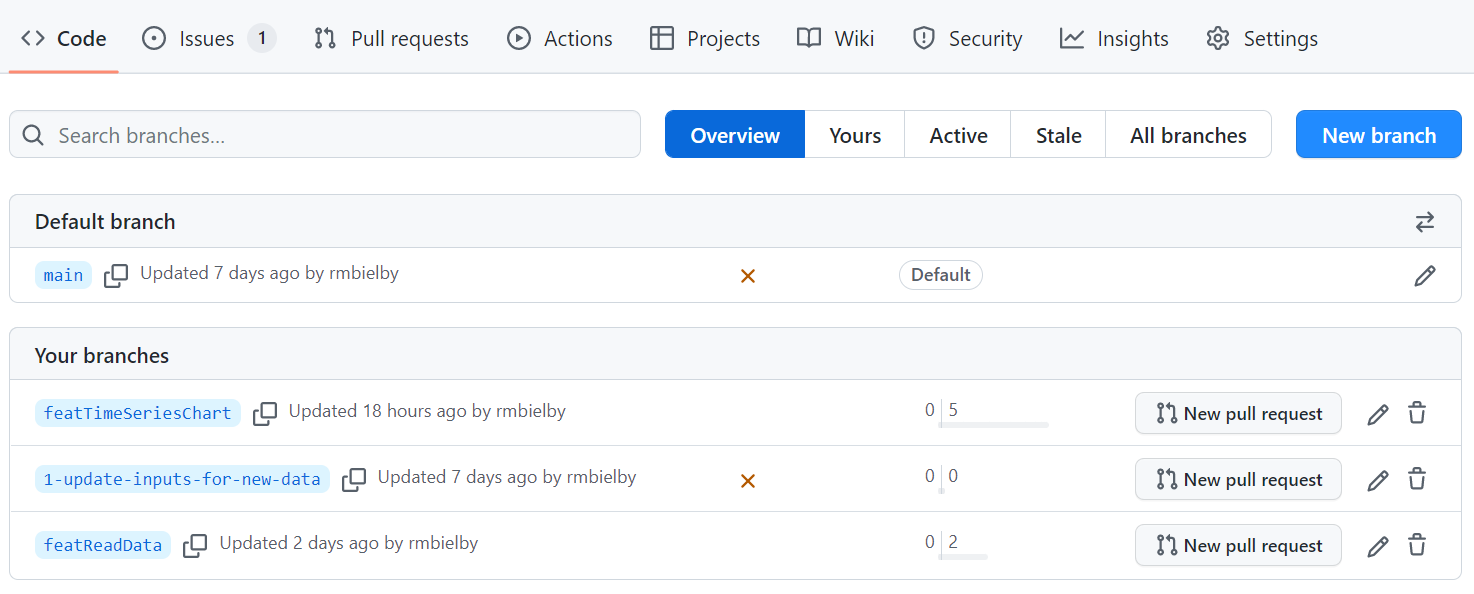
\includegraphics[width=0.64\linewidth]{images/gitdemo/gitdemo-GitHub-Branches} 

}

\caption{The branches overview pane in GitHub.}\label{fig:unnamed-chunk-15}
\end{figure}

Click \textbf{New pull request} on the branch for task 1c, which now
contains all the updates. That will open up the pull request page, where
you can give some details for collaborators to understand what's in this
update to the code. The pull request will default to performing a merge
from the branch you've created it on into the \emph{main} branch.

\begin{figure}

{\centering 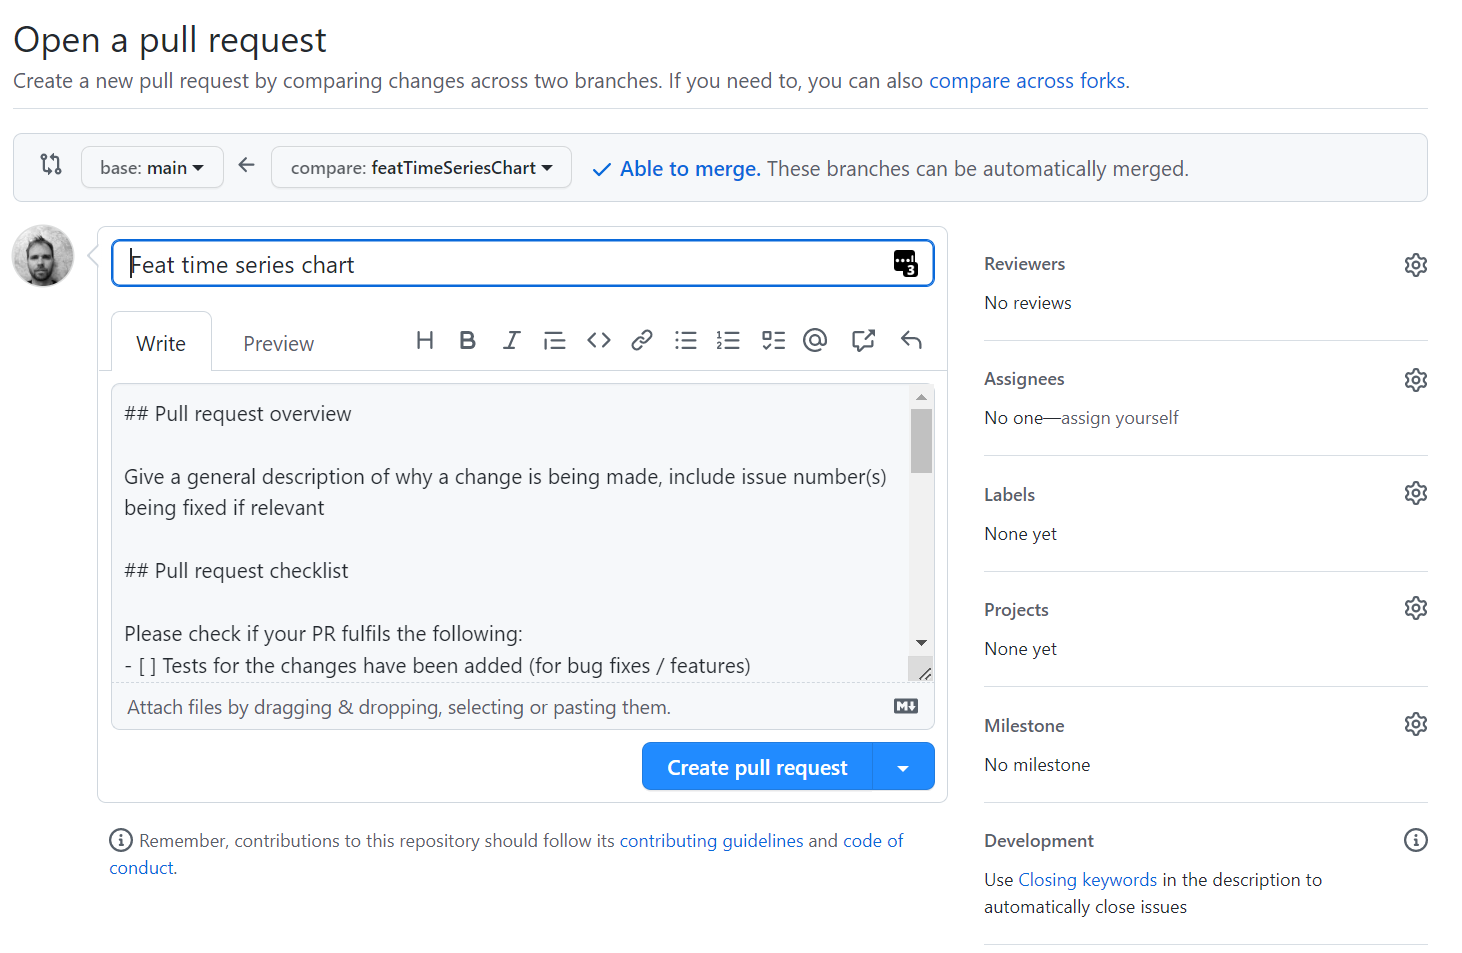
\includegraphics[width=0.64\linewidth]{images/gitdemo/gitdemo-GitHub-OpenPullRequest} 

}

\caption{Opening a Pull Request on GitHub.}\label{fig:unnamed-chunk-16}
\end{figure}

There are a few useful things to do here:

\begin{enumerate}
\def\labelenumi{\arabic{enumi}.}
\tightlist
\item
  Give the PR a meaningful title.
\item
  Give it a meaningful description so collaborators know what change in
  the project you're aiming for. You can also link to issues here, for
  example by saying ``This PR closes \#1'' (where \#1 is the issue
  reference).
\item
  Assign reviewers - add the other members of your group here!
\end{enumerate}

Once you've filled in those elements, you can click \textbf{Create pull
request}. Note that this won't merge the branch into main, this just
creates a review area where you can access useful info on the merge and
get feedback from collaborators.

\hypertarget{reviewing-a-pull-request}{%
\subsubsection{Reviewing a pull
request}\label{reviewing-a-pull-request}}

There are some basic steps to go through if you're asked to review a
pull request. The key elements are:

\begin{enumerate}
\def\labelenumi{\arabic{enumi}.}
\tightlist
\item
  Review any automated checks or QA scripts;
\item
  Clone the repository, switch to the relevant branch and run the code;
\item
  Look through and comment on the changes to the repository using the
  \textbf{Files changes} panel in the PR.
\end{enumerate}

In this case, we don't have any automated checks set up properly, so
we'll focus on points 2 and 3.

First of all try switching to the \emph{featTimeSeriesChart} branch if
you're not already in it and run the Shiny app - this can be done by
opening the global.R script in RStudio and clicking Run App in the top
right hand corner of the viewer pane. Assuming the dashboard runs, then
try cycling through the different panels of the dashboard looking for
any problems, errors or just things that could be improved.

There should be plenty of issues to find as we've kept the actual
dashboard coding brief to focus on using git. As you find them, enter
them in to the GitHub pull request, either under \textbf{Review changes}
on the Files changed panel or as comments in the \textbf{Conversation}
panel.

In reality, once you've got those reviews collated, you'd go through and
make changes to the code accordingly. This provides the checks and
balances and a structure for code QA necessary when developing
reproducible analyticle pipelines or data dashboards.

Assuming we've dealt with the outcomes of those reviews appropriately,
the next step is to complete the Pull request by clicking the
\textbf{Merge pull request} button. This then completes the merge in to
\emph{main} in this case. Whilst the basic mechanics of what's happening
with the branches is the same here as with just running
\texttt{git\ merge}, the Pull request provides that extra layer of
administrative structure to perform proper QA of the code and the
resulting product.

\hypertarget{merge-conflicts}{%
\subsection{Merge conflicts}\label{merge-conflicts}}

When \texttt{git} performs a merge, it uses the histories of different
changes that were made to files to help understand what changes in any
given file supersede other across a pair of branches. In some cases, for
example of two branches contain contradictory changes to the same part
of a file, then \texttt{git} won't automatically merge the two versions
of that file and will instead call for the user to give it some steer on
how it should procede. This is called a \textbf{merge conflict}.

\hypertarget{summary-1}{%
\subsection{Summary}\label{summary-1}}

We've looked through a lot of the basics in this section, covering
adding/staging, committing, pushing/pulling between remote and local
repos, merging and pull requests. These are all the main concepts you
need to use git.

We've also tried to cover doing all this through a mixture of RStudio,
git BASH and GitHub (and as we've said Azure Dev Ops offers similar
functionality to GitHub). Most common processes can be done multiple
ways and there's not necessarily a single right method to follow, just
whichever makes most sense in your situation.

Just a quick final note on why it's useful to be familiar with git
\texttt{BASH}. Whilst most of the basic git functionality can be
accessed via the RStudio interface or GitHub/Dev Ops, there are some
things that are best achieved through BASH. In particular, if you have a
file in your repo that you need to remove entirely, this pretty much
requires someone to use commands via git BASH.

\begin{longtable}[]{@{}
  >{\raggedright\arraybackslash}p{(\columnwidth - 4\tabcolsep) * \real{0.2113}}
  >{\raggedright\arraybackslash}p{(\columnwidth - 4\tabcolsep) * \real{0.4225}}
  >{\centering\arraybackslash}p{(\columnwidth - 4\tabcolsep) * \real{0.3662}}@{}}
\toprule()
\begin{minipage}[b]{\linewidth}\raggedright
Process
\end{minipage} & \begin{minipage}[b]{\linewidth}\raggedright
git BASH
\end{minipage} & \begin{minipage}[b]{\linewidth}\centering
RStudio git panel
\end{minipage} \\
\midrule()
\endhead
Create branch & \texttt{git\ checkout\ -b\ branch\_name} &
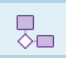
\includegraphics{"images/gitdemo/gitdemo-RStudio-gitToolbarCreateBranch.png"} \\
Switch branch & \texttt{git\ checkout\ branch\_name} &

\includegraphics{"images/gitdemo/gitdemo-RStudio-gitToolbarSwitchBranch.png"} \\
Merge branch & \texttt{git\ merge\ branch\_name} & N/A - use GitHub/Dev
Ops \\
\bottomrule()
\end{longtable}

\newpage

\hypertarget{troubleshooting}{%
\section{Troubleshooting}\label{troubleshooting}}

\hypertarget{renv}{%
\subsection{renv}\label{renv}}

If \texttt{renv::restore()} causes issues, then one of your team should
try \texttt{renv::init()} and select option 2 to restart renv. Then do a
add/commit/push cycle and get the other team members to do a pull and
then try running \texttt{renv::restore()} again on their local clones of
the repo.

\hypertarget{datafiles-commit-hooks.gitignore}{%
\subsection{\texorpdfstring{Datafiles
commit-hooks/\texttt{.gitignore}}{Datafiles commit-hooks/.gitignore}}\label{datafiles-commit-hooks.gitignore}}

To help teams keep on top of avoiding any accidental publishing of
unpublished data, we've added in some code around commits that checks
through any data files in the repo and checks them against a logfile and
the .gitignore file. Any files listed in .gitignore will not be included
in commits and therefore won't be sent to the remote repo as part of any
push.

\hypertarget{merge-conflicts-1}{%
\subsection{merge conflicts}\label{merge-conflicts-1}}

Merge commits happen when two branches have conflicting changes that
have been made concurrently. \texttt{git} can usually figure out how to
prioritise changes based on the commit history, but if changes have
happened at the same time to the same bit of code across different
branches, then it will need to get your input on how to prioritise the
changes.

The easiest way to go through how to deal with merge conflicts is by
discussing with an example, so ask us in the workshop if and when you
hit a merge conflict.

Briefly though, when there's a merge conflict, git will add some text to
the file containing the conflict along the following lines:

\begin{verbatim}
<<<<<<<<<<< branch_1
code 
on 
branch 
1
===========
conflicting code on branch 2
>>>>>>>>>>> branch_2
\end{verbatim}

Effectively as the user, you need to decide which bit of code is the
right bit to keep and then delete anything you don't want to keep as
well as the tag-lines that git has added in. So for example, you should
be left with something along the lines of:

\begin{verbatim}
code 
on 
branch 
1
\end{verbatim}

Once you've cleared up all merge conflicts in the branch that you're
working on, then perform another add/commit cycle and thay should clear
out the conflict from the branch that you're working on and you'll be
able to continue with the intended merge/PR.

\newpage

\resizebox{48mm}{!}{
\includegraphics{images/Department_for_Education.png}}
\vspace*{\fill}
\color{black}

© Crown copyright 2022

This publication (not including logos) is licensed under the terms of
the Open Government Licence v3.0 except where otherwise stated. Where we
have identified any third party copyright information you will need to
obtain permission from the copyright holders concerned.

To view this licence:

\begin{tabular}{p{0.02\linewidth} p{0.1\linewidth} p{0.88\linewidth}}
& visit & www.nationalarchives.gov.uk/doc/open-government-licence/version/3 \\
& email & psi@nationalarchives.gsi.gov.uk \\
& write to & Information Policy Team, The National Archives, Kew, London, TW9 4DU \\
\end{tabular}

About this publication:

\begin{tabular}{p{0.02\linewidth} p{0.1\linewidth} p{0.88\linewidth}}
& enquiries & www.education.gov.uk/contactus \\
& download & www.gov.uk/government/publications \\
\end{tabular}

\begin{tabular}[t]{p{0.06\linewidth} p{0.24\linewidth} p{0.04\linewidth} p{0.06\linewidth} p{0.36\linewidth}}
\raisebox{-.5\height}{
\includegraphics{images/logoTwitter.png}} &
Follow us on Twitter: @educationgovuk &
&
\raisebox{-.5\height}{
\includegraphics{images/logoFacebook.png}} &
Like us on Facebook: \qquad facebook.com/educationgovuk\\
\end{tabular}

\end{document}
